\documentclass[a5paper]{article}
\usepackage[a5paper, top=8mm, bottom=8mm, left=8mm, right=8mm]{geometry}

\usepackage{polyglossia}
\setdefaultlanguage[babelshorthands=true]{russian}

\usepackage{fontspec}
\setmainfont{FreeSerif}
\newfontfamily{\russianfonttt}[Scale=0.7]{DejaVuSansMono}

\usepackage[font=scriptsize]{caption}

\usepackage{amsmath}
\usepackage{amssymb,amsfonts,textcomp}
\usepackage{color}
\usepackage{array}
\usepackage{hhline}
\usepackage{cite}

\usepackage[hang,multiple]{footmisc}
\renewcommand{\footnotelayout}{\raggedright}

\PassOptionsToPackage{hyphens}{url}\usepackage[xetex,linktocpage=true,plainpages=false,pdfpagelabels=false]{hyperref}
\hypersetup{colorlinks=true, linkcolor=blue, citecolor=blue, filecolor=blue, urlcolor=blue, pdftitle=1, pdfauthor=, pdfsubject=, pdfkeywords=}

\usepackage{tabu}

\usepackage{graphicx}
\usepackage{indentfirst}
\usepackage{multirow}
\usepackage{subfig}
\usepackage{footnote}
\usepackage{minted}

\sloppy
\pagestyle{plain}

\title{Практика 13: RabbitMQ}
\author{Юрий Литвинов\\\small{yurii.litvinov@gmail.com}}

\date{18.04.2022}

\begin{document}

\maketitle
\thispagestyle{empty}

\section{Введение}

Новички в распределённых приложениях часто думают, что клиент и сервер обычно соединяются друг с другом напрямую, и это даже правда для большого количества веб-сервисов. Однако часто это может приводить к неприятным ошибкам просто из-за кратковременных сетевых отказов, а часто просто не нужно --- мы хотим всего лишь отправить сообщение в надежде, что оно будет обработано когда-то в будущем (например, послать нотификацию по почте --- сейчас или через полчаса, в случае с электронной почтой обычно разницы нет). В качестве прослойки между клиентом и сервером можно использовать очереди сообщений --- системы, обеспечивающие гарантированную доставку сообщений, даже если отправитель и получатель в разное время находятся в онлайне. Обычно очередь сообщений --- это отдельный сервер (который простой и не самодельный, поэтому, скорее всего, у него будет высокий аптайм), либо локальное хранилище сообщений у каждого отправителя. Отправитель не шлёт сообщение непосредственно серверу, а кладёт его в очередь, и сервер, когда готов, забирает его оттуда (либо очередь сама время от времени пытается его доставить, в зависимости от архитектуры конкретной системы).

Очереди сообщений позволяют нескольким отправителям писать сообщения, и нескольким получателям, соответственно, читать, так что позволяют организовать более интересные способы взаимодействия, чем <<точка-точка>> (хотя в этом качестве тоже активно используются). Например, очередь сообщений может реализовывать модель <<издатель-подписчик>>, когда один источник кидает в неё события, а несколько подписчиков вычитывают (при этом, в зависимости от задачи, одно сообщение может доставляться всем подписчикам, а может и только одному --- так, например, можно балансировать нагрузку в распределённых вычислительных системах). Очередь также может выступать в роли шины событий для событийно-ориентированных архитектур --- все, кто производят события, пишут события в очередь (может, в несколько разных очередей, по одной на каждый тип события), все, кто хочет слушать события, просто забирают их из очереди (опять-таки, удаляя событие из очереди или нет).

Очереди при этом обычно имеют развитые возможности по маршрутизации, фильтрации и преобразованию сообщений, реализованные на стороне собственно очереди. Например, разветвители, которые раскидывают сообщения из одной очереди по нескольким, агрегаторы, которые, наоборот, сливают сообщения из нескольких очередей в одну, преобразователи порядка, которые могут переставлять или сортировать сообщения.

RabbitMQ\footnote{Домашняя страница RabbitMQ, \url{https://www.rabbitmq.com/} (дата обращения: 16.04.2022).} --- одна из самых популярных (наряду с Apache Kafka) реализаций очереди сообщений. Это как раз реализация с отдельным сервером (написанным, внезапно, на Erlang, так что чтобы RabbitMQ заработала, ей нужен Erlang runtime). Клиент при отправке сообщения подключается по сети к серверу (никто не мешает задеплоить его на той же машине, что и клиент, впрочем) и сохраняет сообщение там. Сообщение хранится, возможно, будучи записанным на диск, чтобы пережить даже перезапуск сервера RabbitMQ. Когда получатель готов его обработать, он подключается к серверу, указывает из какой очереди забрать сообщение и удалить ли его после обработки, и забирает сообщение. RabbitMQ никакой кодогенерации не использует, сообщения для неё --- просто массивы байтов (что, кстати, даёт возможность сериализовать сообщения в любой формат, например модный нынче protobuf). Клиентские библиотеки доступны практически для любых языков программирования.

RabbitMQ реализует стандартный протокол AMQP (Advanced Message Queuing Protocol), так что теоретически может работать и со сторонними клиентами, но не уверен, что кто-то пробовал. RabbitMQ имеет развитые возможности по маршрутизации сообщений --- на самом деле, сообщение добавляется не в очередь вовсе, а в Exchange --- именованный и конфигурируемый маршрутизатор, который по умолчанию тут же пересылает сообщение в очередь с таким же именем и больше ничего не делает (так что пользоваться RabbitMQ можно, даже не зная про существование exchange-ей). Однако ему можно сказать раскидывать сообщения по разным очередям, маршрутизировать сообщения по ключам, отправляемым с сообщением клиентом, фильтровать сообщения и творить прочие хорошие вещи.

\section{Архитектура}

Концептуально RabbitMQ устроена очень просто:

\begin{center}
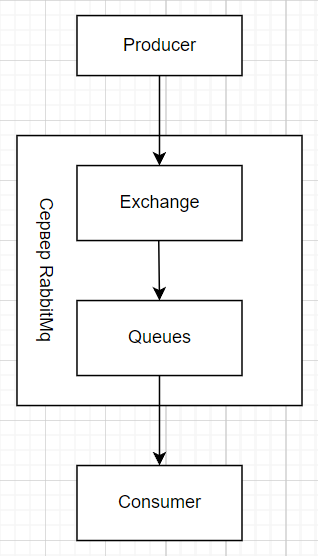
\includegraphics[width=0.3\textwidth]{rabbitMqArchitecture.png}
\end{center}

\begin{itemize}
    \item Producer --- это код клиентского приложения, который использует соответствующую клиентскую библиотеку. Он отправляет сообщения в очередь. 
    \item Exchange маршрутизует сообщения, в зависимости от самого сообщения (точнее, его поля <<routing key>> --- чего-то вроде строкового тэга/тэгов сообщения) и от настроек Exchange-а.
    \item Queue хранит сообщения и выдаёт клиентам по запросу. Обработанное сообщение удаляется из очереди (что принципиально отличает RabbitMQ от Apache Kafka, где сообщения не удаляются). На одну очередь может подписаться несколько клиентов, тогда сообщение будет доставляться каждому по очереди, часто также каждому клиенту соответствует своя очередь, тогда Exchange может раскопировать сообщение в них.
    \item Consumer --- это код клиентского приложения, который забирает сообщение из очереди. Обычно в клиентской библиотеке используются коллбэки или события, которые дёргаются при появлении события в очереди на сервере, обычно это происходит асинхронно (хотя тут могут быть неожиданности, надо смотреть документацию клиентской библиотеки для вашего языка).
\end{itemize}

Вот пример ситуации, когда Exchange копирует сообщение в несколько клиентских очередей, тем самым доставляя его всем клиентам сразу (тип exchange --- fanout):

\begin{center}
    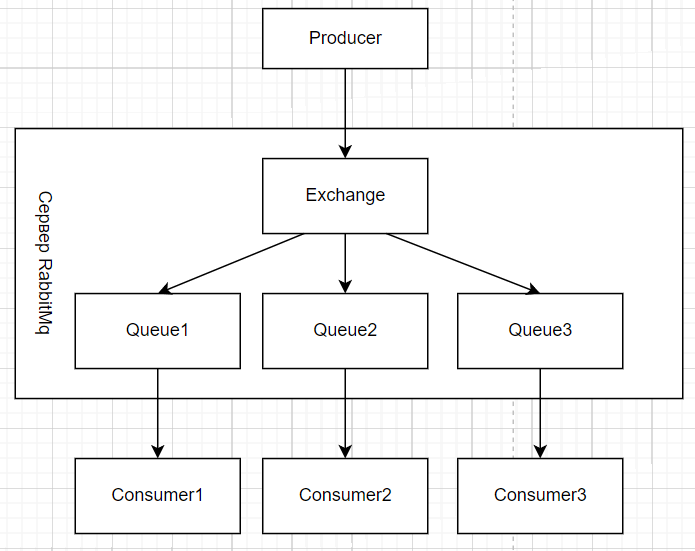
\includegraphics[width=0.6\textwidth]{fanoutExchange.png}
\end{center}

А вот пример более сложной ситуации, когда Exchange маршрутизует сообщение в зависимости от их routing key (тип --- direct exchange). routing key в этом случае должен быть не произвольной строкой, а иметь вид <<слово.слово.слово...>>, а настройки exchange должны содержать шаблон с конкретными словами, \verb|*|, которая матчит любое слово или \verb|#|, которая матчит сколько угодно слов. Routing key должен указываться producer-ом для каждого сообщения при отправке:

\begin{center}
    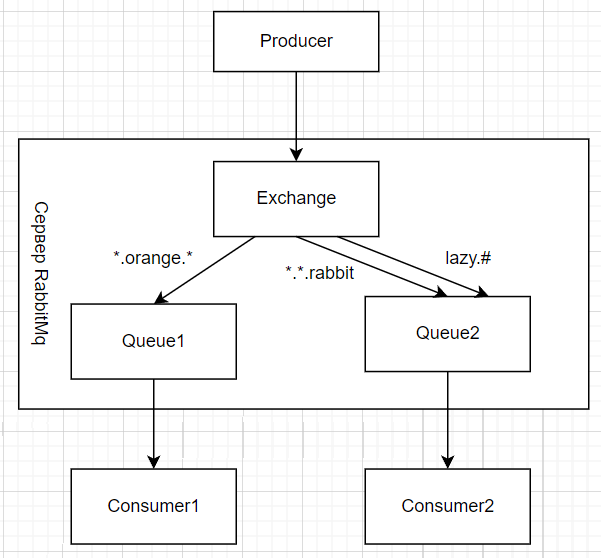
\includegraphics[width=0.6\textwidth]{topicExchange.png}
\end{center}

\section{Пример}

Наконец перейдём к примеру кода. Вот отправитель (на C\#):

\begin{minted}{csharp}
using RabbitMQ.Client;
using System.Text;

var factory = new ConnectionFactory() { HostName = "localhost" };
using var connection = factory.CreateConnection();
using var channel = connection.CreateModel();

channel.QueueDeclare(queue: "hello",
    durable: false,
    exclusive: false,
    autoDelete: false,
    arguments: null);

var message = "Hello World!";
var body = Encoding.UTF8.GetBytes(message);

channel.BasicPublish(exchange: "",
    routingKey: "hello",
    basicProperties: null,
    body: body);

Console.WriteLine($" [x] Sent {message}");
\end{minted}

Создаём подключение, сообщая ConnectionFactory имя хоста, на котором запущен сервер. Порт указывать не надо, он по умолчанию 5672. Дальше создаём канал --- канал представляет виртуальное соединение по протоколу AMPQ внутри физического подключения, которое описывается классом Connection. Теоретически один Connection может поддерживать несколько каналов. Дальше мы внутри канала объявляем очередь с именем <<hello>>, говорим (durable: false), что она должна сохранять сообщения только в память, а не на диск (так менее надёжно, но быстрее), что очередь не надо удалять при закрытии соединения (exclusive: false), что очередь не надо удалять, когда читатель от неё отписывается (autoDelete: false), не передаём дополнительных аргументов. Если очередь с таким именем на сервере уже есть, QueueDeclare ничего не делает, однако если параметры очереди не совпадают, RabbitMQ вернёт ошибку. Дальше мы сериализуем наше сообщение и публикуем его в очередь (методом BasicPublish) с ключом <<hello>>, по которому exchange поймёт, что его надо отправить в очередь <<hello>>.

Теперь получатель:

\begin{minted}{csharp}
using RabbitMQ.Client;
using RabbitMQ.Client.Events;
using System.Text;

var factory = new ConnectionFactory() { HostName = "localhost" };
using var connection = factory.CreateConnection();
using var channel = connection.CreateModel();

channel.QueueDeclare(queue: "hello",
    durable: false,
    exclusive: false,
    autoDelete: false,
    arguments: null);

var consumer = new EventingBasicConsumer(channel);

consumer.Received += (model, ea) =>
{
var body = ea.Body.ToArray();
var message = Encoding.UTF8.GetString(body);
Console.WriteLine($" [x] Received {message}");
};

channel.BasicConsume(queue: "hello",
    autoAck: true,
    consumer: consumer);
\end{minted}

Тут тоже, создаём подключение к локалхосту, объявляем очередь (на случай, если получатель будет запущен раньше отправителя, если нет, то QueueDeclare ничего не делает). А дальше мы создаём асинхронного получателя сообщений и запускаем блокирующий метод BasicConsume, указывая ему очередь, которую надо слушать, автоматически подтверждать доставку и удалять сообщение из очереди, ну и consumer, который будет вызываться при появлении в очереди сообщения. Собственно получатель --- это лямбда-функция с двумя аргументами, подписанная на событие Received у consumer. model --- это канал, ea --- собственно полученное сообщение, у него мы берём тело (байтовый массив), десериализуем и печатаем на экран.

Обратите внимание, это прямо готовые программы отправителя и получателя, да и сам RabbitMQ с параметрами по умолчанию запустить ничего не стоит (особенно из Docker-контейнера), так что завести это всё в базовом варианте --- дело десяти минут. Впрочем, правильно всё настроить (например, авторизацию по сертификатам --- вы же не хотите, чтобы кто угодно мог подписываться на сообщения или писать сообщения в очередь) может быть уже не так тривиально. Например, прямо из коробки RabbitMQ будет отклонять запросы с другого хоста без авторизации, так что локально у вас может всё работать, а как только вы подумаете, что у нас же распределённое приложение и давайте попробуем подключить клиента с другой машины --- получите ошибку.

И наконец, как всё собрать и запустить:

\begin{itemize}
    \item поставить сервер RabbitMQ, инструкции по установке есть на \url{https://www.rabbitmq.com/download.html};
    \item проще всего воспользоваться docker-образом, но если не умеете, то ставить лучше из менеджера пакетов, иначе потребуется сначала руками поставить рантайм Erlang;
    \item добавить зависимость от клиента RabbitMQ в проект:
    \begin{itemize}
        \item в .NET: добавить RabbitMQ.Client через менеджер пакетов NuGet (в Visual Studio, например, это Manage NuGet Packages в меню по правому клику по проекту --- обратите внимание, по проекту (project), не по решению (solution));
        \item в JVM через Gradle: \mintinline{groovy}|compile group: 'com.rabbitmq', name: 'amqp-client', version: '5.14.2'|;
    \end{itemize}
    \item по идее всё, но стоит также пролистать Getting Started для вашего любимого языка: \url{https://www.rabbitmq.com/getstarted.html}, часть 1
\end{itemize}

\section{Задача}

Задачей на практику будет в командах по два-три человека реализовать консольный сетевой чат на RabbitMQ. Считаем, что сервер для обмена сообщениями (то есть сам RabbitMQ, не нужно самодельный сервер) развёрнут в известном всем клиентам месте. По умолчанию это 127.0.0.1, но должна быть возможность параметром командной строки указать другой IP-адрес. Порт не надо, используется порт по умолчанию (5672). Чат запускается и запускает REPL, где можно писать сообщения, и они должны отправляться всем получателям.

Вместо списка контактов есть именованные каналы, на которые можно переключаться и постить туда. Начальный канал принимаем как аргумент командной строки, переключаться на другие каналы должно быть можно с помощью консольной команды (например, что-то вроде <<!switch channel1>>). Переключение на несуществующий канал должно его создавать. Переключение обратно на какой-то канал должно показывать все сообщения, которые были в этом канале с момента нашего от него отключения. Получать сообщения, отправленные пока мы были в оффлайне, не обязательно.

Может быть полезен туториал по диспетчеризации по exchange-ам --- \url{https://www.rabbitmq.com/tutorials/tutorial-three-dotnet.html}. Но задача вообще предполагает большое количество разбирательства в документации, не только в туториале.

\end{document}
